\section{SPI}
\subsection{Protocol Overview}
SPI stands for Serial Peripheral Interface. Serial Peripheral Interface (SPI) is one of the most widely used interfaces between microcontroller and peripheral ICs such as sensors, ADCs, DACs, shift registers, SRAM, and others. SPI is a synchronous, full duplex master-slave-based interface. The SPI interface can be either 3-wire or 4-wire.

\begin{figure}[H]
\begin{center}
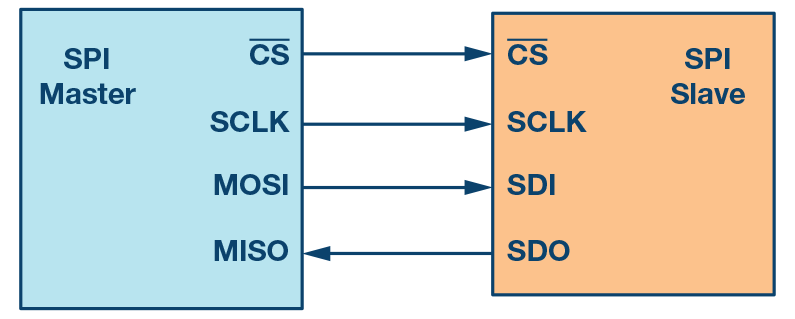
\includegraphics[width=4in]{images/SPI.png}
\caption{SPI Protocol Overview}
\label{SPI}
\end{center}
\end{figure} 

4-wire SPI devices have four signals:
\begin{enumerate}
    \item Clock (SPI CLK, SCLK)
    \item Chip select (CS)
    \item Master out, slave in (MOSI)
    \item Master in, slave out (MISO)
\end{enumerate}

The device that generates the clock signal is called the Master. Data transmitted between the master and the slave is synchronized to the clock generated by the master. The data from the master or the slave is synchronized on the rising or falling clock edge. Both master and slave can transmit data at the same time. SPI devices support much higher clock frequencies compared to I2C interfaces. SPI interfaces can have only one master and can have one or multiple slaves. MOSI and MISO are the data lines. MOSI transmits data from the master to the slave and MISO transmits data from the slave to the master. The chip select signal from the master is used to select the slave. This is normally an active low signal and is pulled high to disconnect the slave from the SPI bus. When multiple slaves are used, an individual chip select signal for each slave is required from the master. 

\subsection{Data Transmission}
To begin SPI communication, the master must send the clock signal and select the slave by enabling the CS signal. Usually chip select is an active low signal. Hence, the master must send a logic 0 on this signal to select the slave. SPI is a full-duplex interface both master and slave can send data at the same time via the MOSI and MISO lines respectively. During SPI communication, the data is simultaneously transmitted (shifted out serially onto the MOSI/SDO bus) and received (the data on the bus (MISO/SDI) is sampled or read in). The serial clock edge synchronizes the shifting and sampling of the data. The SPI interface provides the user with flexibility to select the rising or falling edge of the clock to sample and/or shift the data. Please refer to the device data sheet to determine the number of data bits transmitted using the SPI interface.

\clearpage
\subsection{Clock Polarity and Clock Phase}
In SPI, the master can select the clock polarity and clock phase. The CPOL bit sets the polarity of the clock signal during the idle state. The idle state is defined as the period when CS is high and transitioning to low at the start of the transmission and when CS is low and transitioning to high at the end of the transmission. The CPHA bit selects the clock phase. Depending on the CPHA bit, the rising or falling clock edge is used to sample and/or shift the data. The master must select the clock polarity and clock phase, as per the requirement of the slave. Depending on the CPOL and CPHA bit selection, four SPI modes are available. 

\begin{table}[H]
    \begin{center}
    \resizebox{\textwidth}{!}{
    \begin{tabular}{@{}lllll@{}}
    \toprule
    \textbf{SPI Mode} & \textbf{CPOL} & \textbf{CPHA} & \textbf{Clock Polarity in Idle State} & \textbf{Clock Phase Used to Sample and/or Shift the Data} \\ \midrule
		
     0	& 0	  & 0	& Logic low	  & Data sampled on rising edge and shifted out on the falling edge      \\   
     1	& 0	  & 1	& Logic low	  & Data sampled on the falling edge and shifted out on the rising edge  \\
     2	& 1	  & 1	& Logic high  & Data sampled on the falling edge and shifted out on the rising edge  \\
     3	& 1	  & 0	& Logic high  & Data sampled on the rising edge and shifted out on the falling edge  \\  \bottomrule

    \end{tabular} 
    }   
    \end{center}
\end{table}

\figref{SPIMode0} through \figref{SPIMode3} show an example of communication in four SPI modes. In these examples, the data is shown on the MOSI and MISO line. The start and end of transmission is indicated by the dotted green line, the sampling edge is indicated in orange, and the shifting edge is indicated in blue.\\ 
\figref{SPIMode0} shows the timing diagram for SPI Mode 0. In this mode, clock polarity is 0, which indicates that the idle state of the clock signal is low. The clock phase in this mode is 0, which indicates that the data is sampled on the rising edge and the data is shifted on the falling edge of the clock signal.

\begin{figure}[H]
\begin{center}
    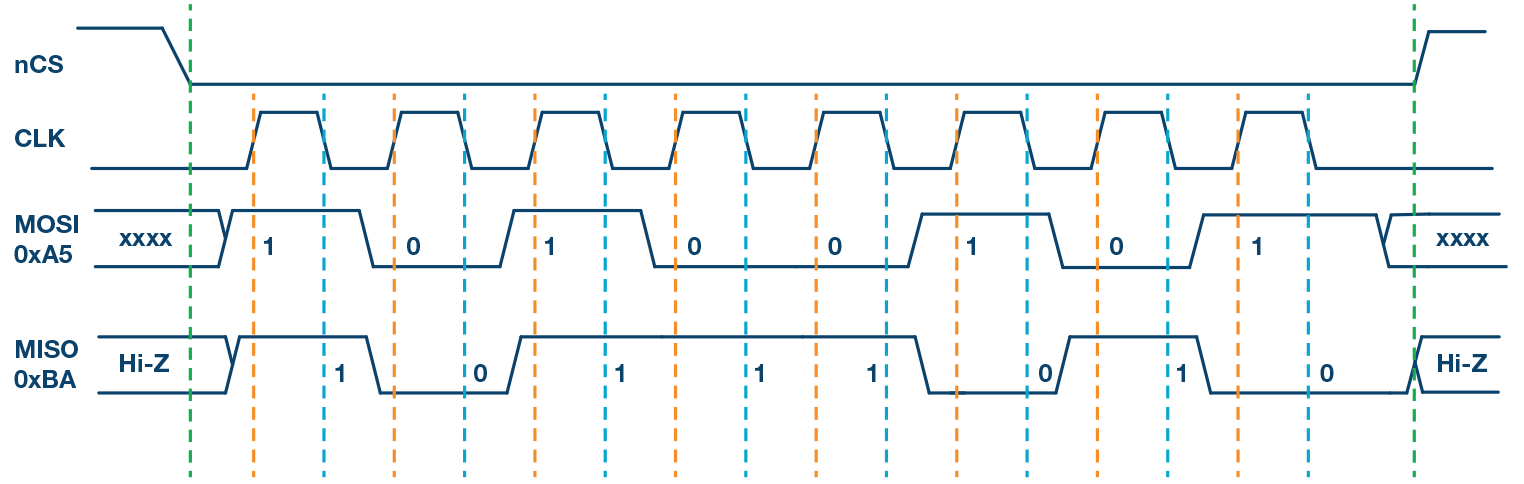
\includegraphics[width=0.9\textwidth]{images/SPIMode0.png} 
    \caption{SPI Mode 0, CPOL = 0, CPHA = 0: CLK idle state = low, data sampled on rising edge and shifted on falling edge.}
    \label{SPIMode0}
\end{center}
\end{figure}

\figref{SPIMode1} shows the timing diagram for SPI Mode 1. In this mode, clock polarity is 0, which indicates that the idle state of the clock signal is low. The clock phase in this mode is 1, which indicates that the data is sampled on the falling edge and the data is shifted on the rising edge of the clock signal.

\begin{figure}[H]
\begin{center}
    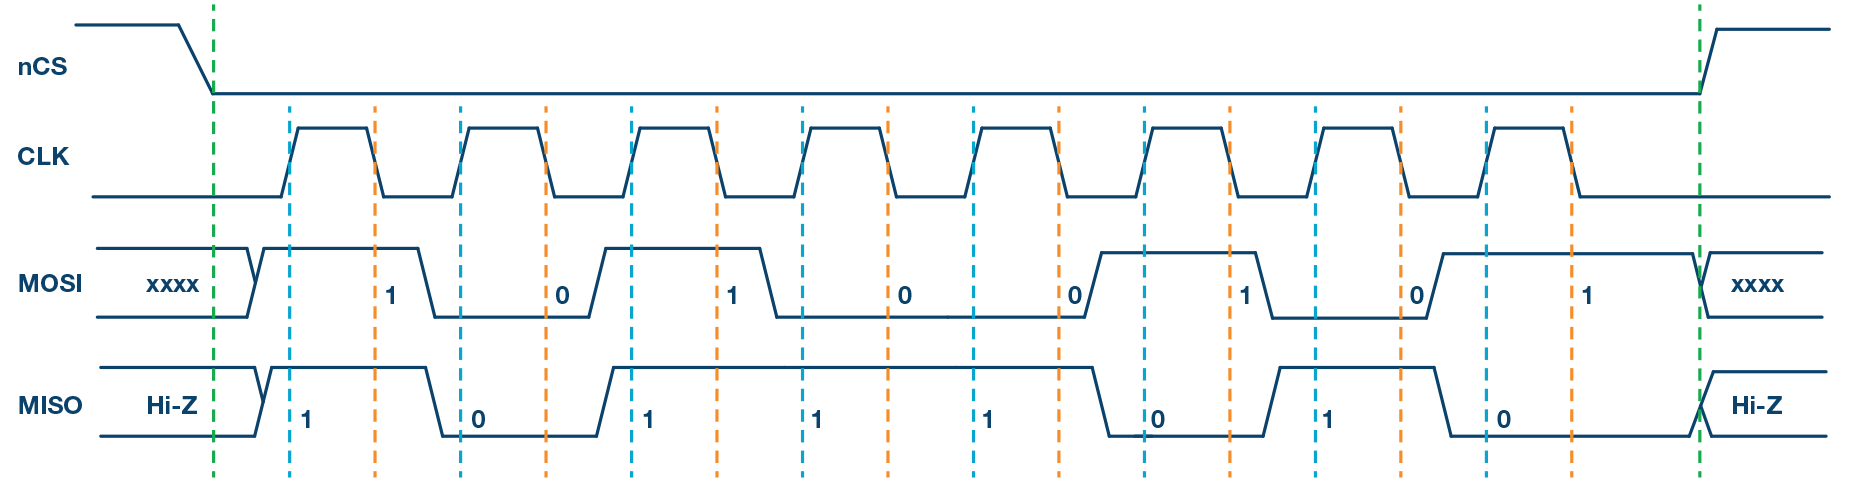
\includegraphics[width=0.9\textwidth]{images/SPIMode1.png} 
    \caption{SPI Mode 1, CPOL = 0, CPHA = 1: CLK idle state = low, data sampled on the falling edge and shifted on the rising edge.}
    \label{SPIMode1}
\end{center}
\end{figure}

\figref{SPIMode2} shows the timing diagram for SPI Mode 2. In this mode, the clock polarity is 1, which indicates that the idle state of the clock signal is high. The clock phase in this mode is 1, which indicates that the data is sampled on the falling edge and the data is shifted on the rising edge of the clock signal.

\begin{figure}[H]
\begin{center}
    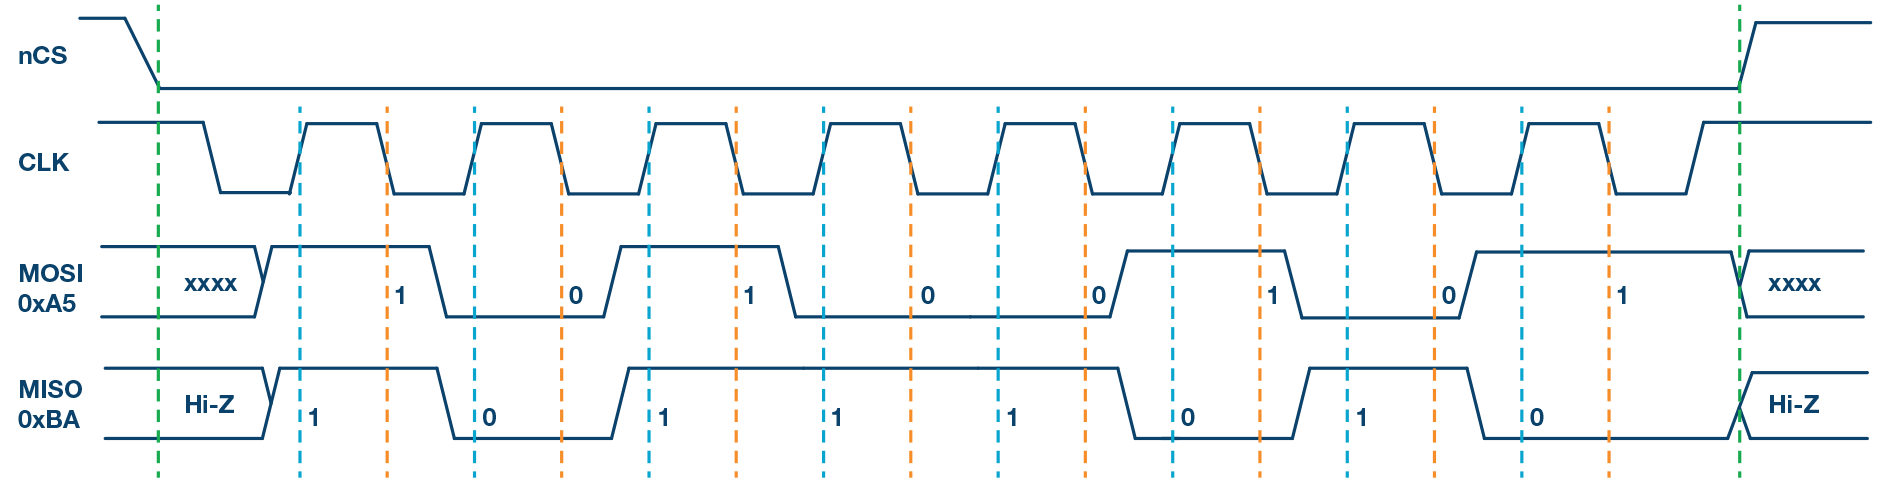
\includegraphics[width=0.9\textwidth]{images/SPIMode2.png} 
    \caption{SPI Mode 2, CPOL = 1, CPHA = 1: CLK idle state = high, data sampled on the falling edge and shifted on the rising edge.}
    \label{SPIMode2}
\end{center}
\end{figure}

\figref{SPIMode3} shows the timing diagram for SPI Mode 3. In this mode, the clock polarity is 1, which indicates that the idle state of the clock signal is high. The clock phase in this mode is 0, which indicates that the data is sampled on the rising edge and the data is shifted on the falling edge of the clock signal.

\begin{figure}[H]
\begin{center}
    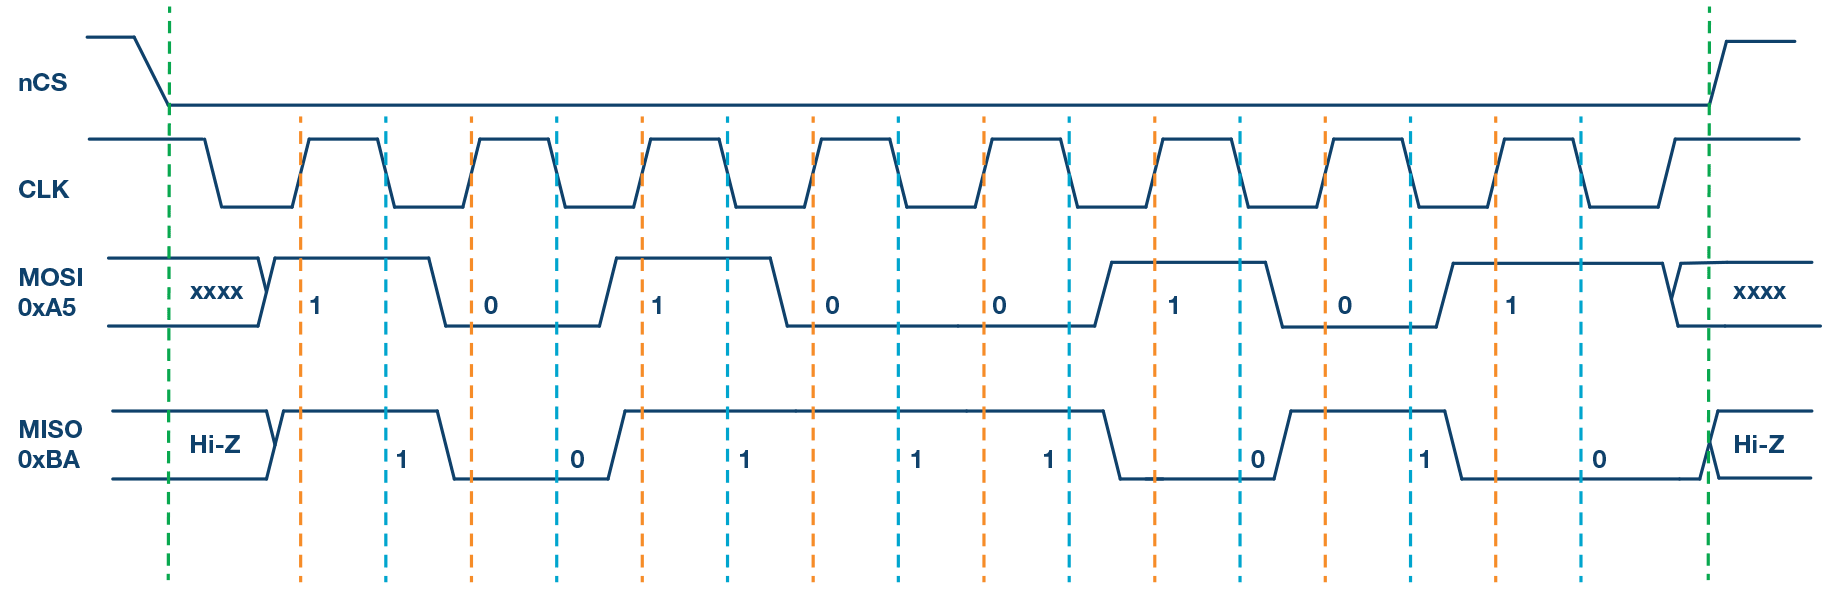
\includegraphics[width=0.9\textwidth]{images/SPIMode3.png} 
    \caption{SPI Mode 3, CPOL = 1, CPHA = 0: CLK idle state = high, data sampled on the rising edge and shifted on the falling edge.}
    \label{SPIMode3}
\end{center}
\end{figure}

\subsection{Multislave Configuration}
Multiple slaves can be used with a single SPI master. The slaves can be connected in regular mode or daisy-chain mode.

\subsubsection{Regular SPI Mode}
\begin{figure}[H]
\begin{center}
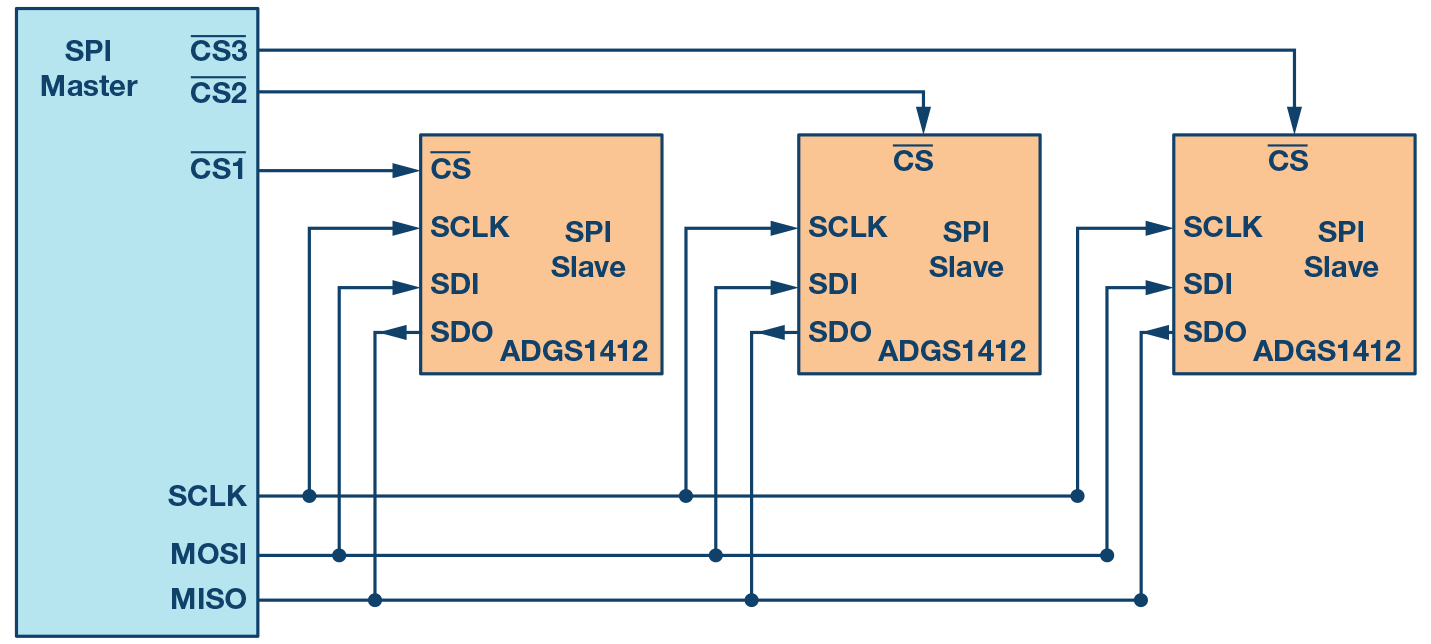
\includegraphics[width=4in]{images/SPIMultiSlave.png}
\caption{Multislave Configuration}
\label{SPIMultiSlave}
\end{center}
\end{figure} 

In regular mode, an individual chip select for each slave is required from the master. Once the chip select signal is enabled (pulled low) by the master, the clock and data on the MOSI/MISO lines are available for the selected slave. If multiple chip select signals are enabled, the data on the MISO line is corrupted, as there is no way for the master to identify which slave is transmitting the data. As the number of slaves increase, the number of chip select lines from the master increase. This can quickly add to the number of inputs and outputs needed from the master and limit the number of slaves that can be used. 

\subsubsection{Daisy-Chain Method}
\begin{figure}[H]
\begin{center}
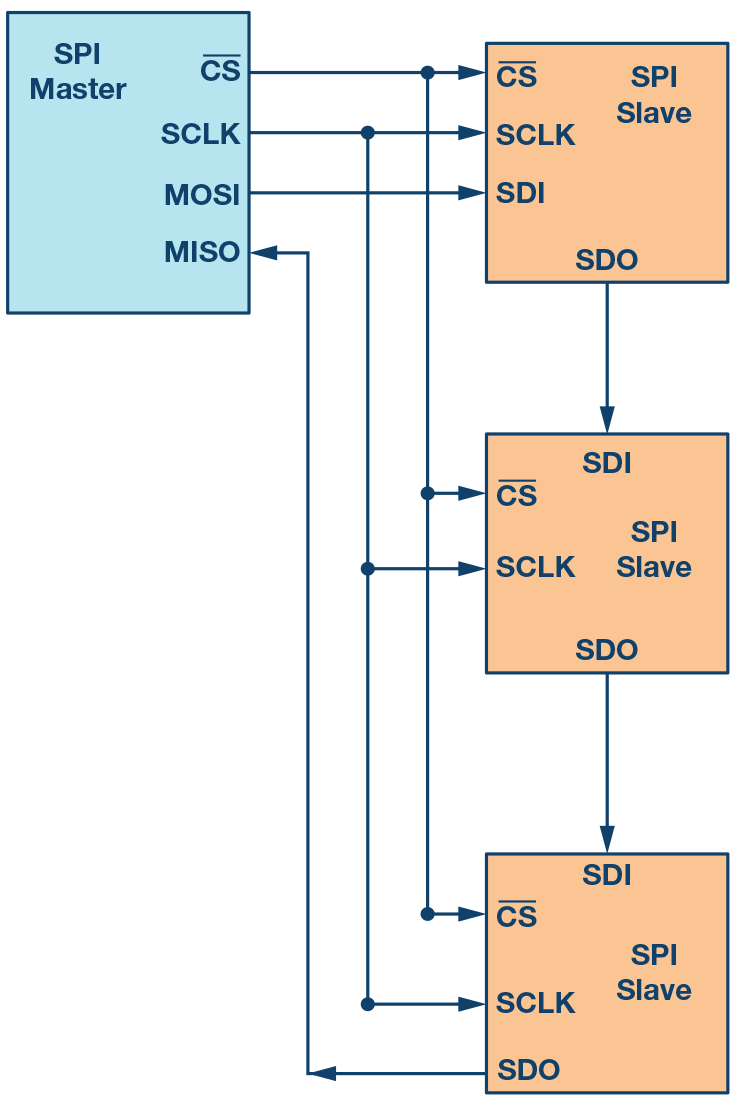
\includegraphics[width=2in]{images/SPIDaisy.png}
\caption{Daisy-Chain Multislave Configuration}
\label{SPIDaisy}
\end{center}
\end{figure} 

In daisy-chain mode, the slaves are configured such that the chip select signal for all slaves is tied together and data propagates from one slave to the next. In this configuration, all slaves receive the same SPI clock at the same time. The data from the master is directly connected to the first slave and that slave provides data to the next slave and so on.

As data is propagated from one slave to the next, the number of clock cycles required to transmit data is proportional to the slave position in the daisy chain. \figref{SPIDaisyTiming} shows the clock cycles and data propagating through the daisy chain. Daisy-chain mode is not necessarily supported by all SPI devices. 

\begin{figure}[H]
\begin{center}
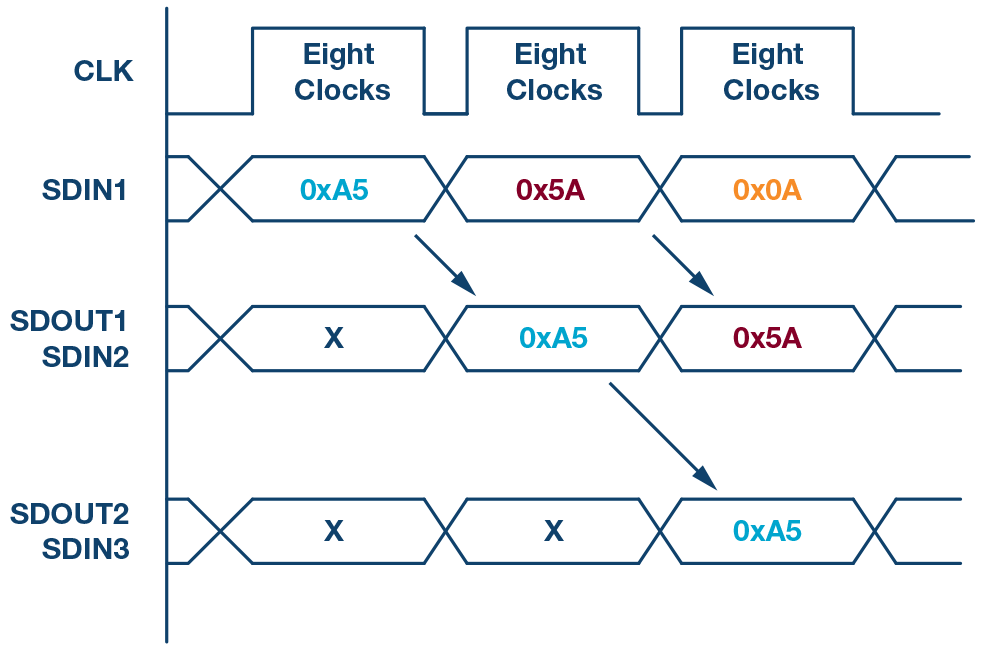
\includegraphics[width=0.5\textwidth]{images/SPIDaisyTiming.png}
\caption{Daisy-chain configuration: data propagation.}
\label{SPIDaisyTiming}
\end{center}
\end{figure} 

\clearpage